\documentclass[paper=a4, oneside]{memoir}

\usepackage[T1]{fontenc}
\usepackage[english]{babel}
\usepackage{amsmath,amsfonts}
\usepackage{tensor}
\usepackage{graphicx}
\usepackage{booktabs}

\usepackage{siunitx}

\chapterstyle{thatcher}

\usepackage{chngcntr}
\counterwithout{table}{chapter}

\graphicspath{{./diagrams/}}


\newcommand{\tens}[2]{\tensor{#1}{#2}}
\newcommand{\packagename}{pichi}


\title{Benchmark tests of certain diagrams}
\author{Christian Walther Andersen\thanks{cwandersen@imada.sdu.dk}}
%\date{}

\begin{document}

\maketitle % Print the title

When doing tensor contractions, we always make a choice of the order in which 
the indices are contracted. This choice can have a large impact on the runtime 
of the contraction code. The intent of this paper is to show the runtime of all 
possible (albeit topologically distinct) choices for all the distinct diagrams 
that we need for hadron spectroscopy. Note that we restrict ourselves here to 
contractions of up to four tensors and only tensors with rank 2 or 3 (mesons 
and baryons).

The result of the benchmark tests are shown in tables \ref{tab1} and 
\ref{tab2}. In the diagrams, an oval is a rank 2 tensor and a triangle is a 
rank 3 tensor, and each vertex is an index. The dotted lines indicate which 
indices are contracted with which. The contraction pattern column shows the 
order of the contractions along with any temporary tensors needed. Every line 
in the contraction pattern is a single \packagename operation. The last 
column shows an estimate of the time it takes to perform the complete 
contraction operation on some machine.

For diagrams 0 through 4 there is only one distinct way to perform the 
contractions. For the rest of the diagrams there are at least two.


\begin{table}[]
	\centering
	\caption{}
	\label{tab1}
	\begin{tabular}{@{}llcll@{}}
		\toprule
	Diagram & \#	& Character rep. & Contraction pattern & Time \\ \midrule
	\parbox{1em}{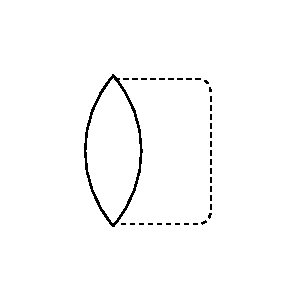
\includegraphics[width=2cm]{Aaa}}& 0 & $\tens{A}{_a_a}$ & 
	$\tens{A}{_a_a}$ & \SI{53(9)}{\micro s} \\
	\parbox{2cm}{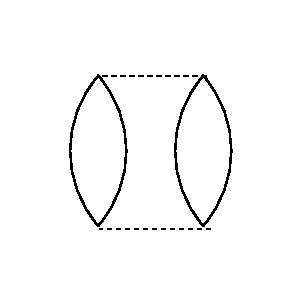
\includegraphics[width=2cm]{AabBab}}& 1 & 
	$\tens{A}{_a_b}\tens{B}{_a_b}$ & $\tens{A}{_a_b}\tens{B}{_a_b}$ & 
	\SI{0.37(10)}{\milli s}\\ 
	\parbox{2cm}{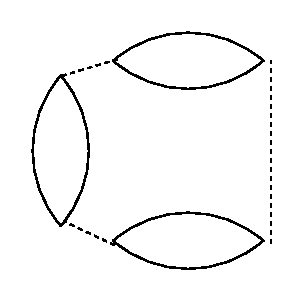
\includegraphics[width=2cm]{AabBbcCac}} & 2& 
	$\tens{A}{_a_b}\tens{B}{_b_c}\tens{C}{_a_c}$ & 
	\parbox[c]{3cm}{$\tens{A}{_a_b}\tens{B}{_b_c} \rightarrow 
	\tens{D}{_a_c}$\\$\tens{D}{_a_c}\tens{C}{_a_c}$}  & 
	\SI{1.3(13)}{\milli s}\\
	\parbox{2cm}{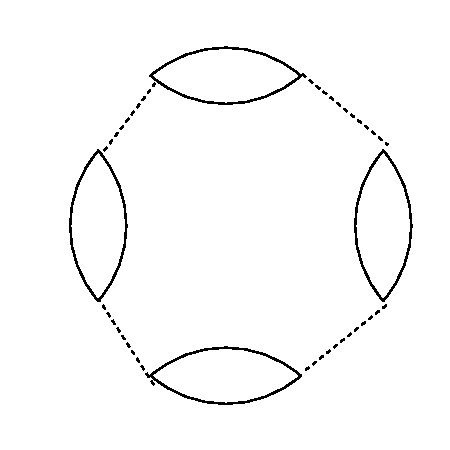
\includegraphics[width=2cm]{AabBbcCcdDad}}& 3 & 
	$\tens{A}{_a_b}\tens{B}{_b_c}\tens{C}{_c_d}\tens{D}{_a_d}$ & 
	\parbox[c]{3cm}{$\tens{A}{_a_b}\tens{B}{_b_c} \rightarrow 
		\tens{E}{_a_c}$\\$\tens{E}{_a_c}\tens{C}{_c_d}\rightarrow 
		\tens{F}{_a_d}$\\$\tens{F}{_a_d}\tens{D}{_a_d}$}  & 
	\SI{1.5(9)}{\milli s}\\
	\parbox{2cm}{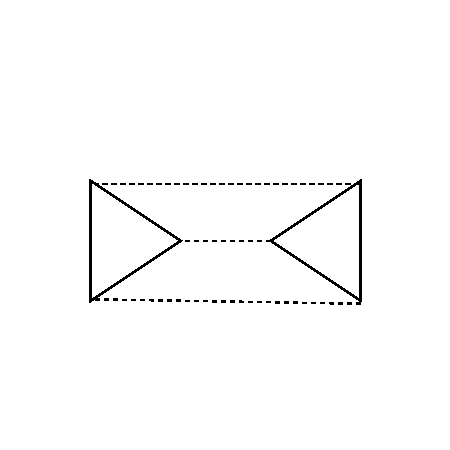
\includegraphics[width=2cm]{AabcBabc}}& 4 & 
	$\tens{A}{_a_b_c}\tens{B}{_a_b_c}$ & 
	\parbox[c]{3cm}{$\tens{A}{_a_b_c}\tens{B}{_a_b_c}$}  & 
	\SI{13.2(7)}{\milli s}\\
	\parbox{2cm}{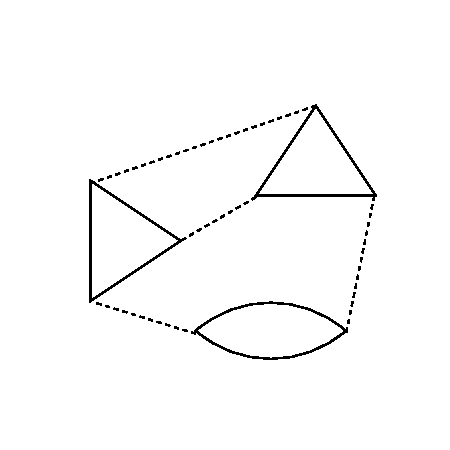
\includegraphics[width=2cm]{AabcBabdCcd}}& 5 & 
	$\tens{A}{_a_b_c}\tens{B}{_a_b_d}\tens{C}{_c_d}$ & 
	\parbox[c]{3cm}{$\tens{A}{_a_b_c}\tens{B}{_a_b_d} \rightarrow 
	\tens{D}{_c_d}$\\$\tens{D}{_c_d}\tens{C}{_c_d}$}  & 
	\SI{0.739(5)}{s}\\
	& 
	& 
	&
	\parbox[c]{3cm}{$\tens{A}{_a_b_c}\tens{C}{_c_d} \rightarrow 
	\tens{D}{_a_b_d}$\\$\tens{D}{_a_b_d}\tens{B}{_a_b_d}$}  & 
	\SI{65(5)}{\milli s}\\
	 \bottomrule
	\end{tabular}
\end{table}

\begin{table}[]
	\centering
	\caption{}
	\label{tab2}
	\begin{tabular}{@{}llcll@{}}
		\toprule
		Diagram	& \# & Character rep. & Contraction pattern & Time \\ \midrule
		\parbox{2cm}{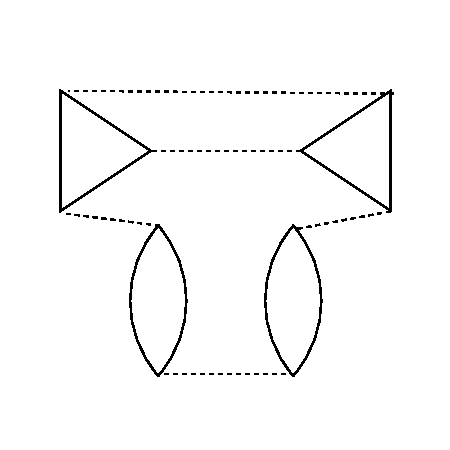
\includegraphics[width=2cm]{AabcBabdCceDde}}& 6 & 
		$\tens{A}{_a_b_c}\tens{B}{_a_b_d}\tens{C}{_c_e}\tens{D}{_d_e}$ & 
		\parbox[c]{3cm}{$\tens{A}{_a_b_c}\tens{B}{_a_b_d} \rightarrow 
			\tens{E}{_c_d}$\\$\tens{E}{_c_d}\tens{C}{_c_e}\rightarrow\tens{F}{_d_e}$\\
			$\tens{F}{_d_e}\tens{D}{_d_e}$}  & 
		\SI{0.738(5)}{s}\\
		& 
		& 
		&
		\parbox[c]{3cm}{$\tens{A}{_a_b_c}\tens{C}{_c_e} \rightarrow 
			\tens{E}{_a_b_e}$\\$\tens{B}{_a_b_d}\tens{D}{_d_e}\rightarrow\tens{F}{_a_b_e}$\\
			$\tens{E}{_a_b_e}\tens{F}{_a_b_e}$}  & 
		\SI{0.119(16)}{s}\\ \\
		& 
		& 
		&
		\parbox[c]{3cm}{$\tens{C}{_c_e}\tens{D}{_d_e} \rightarrow 
			\tens{E}{_c_d}$\\$\tens{A}{_a_b_c}\tens{E}{_c_d}\rightarrow\tens{F}{_a_b_d}$\\
			$\tens{F}{_a_b_d}\tens{B}{_a_b_d}$}  & 
		\SI{68.5(17)}{\milli s}\\
		\parbox{2cm}{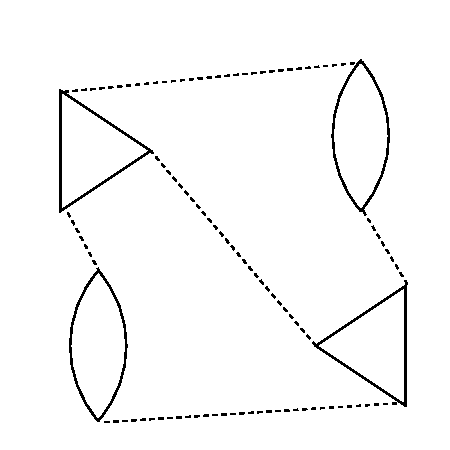
\includegraphics[width=2cm]{AabcBadeCbdDce}}& 7 & 
		$\tens{A}{_a_b_c}\tens{B}{_a_d_e}\tens{C}{_b_d}\tens{D}{_c_e}$ & 
		\parbox[c]{3cm}{$\tens{A}{_a_b_c}\tens{B}{_a_d_e} \rightarrow 
			\tens{E}{_b_c_d_e}$\\$\tens{E}{_b_c_d_e}\tens{C}{_b_d}\rightarrow\tens{F}{_c_e}$\\
			$\tens{F}{_c_e}\tens{D}{_c_e}$}  & 
		\SI{1.88(9)}{s}\\
		& 
		& 
		&
		\parbox[c]{3cm}{$\tens{A}{_a_b_c}\tens{C}{_b_d} \rightarrow 
			\tens{E}{_a_c_d}$\\$\tens{E}{_a_c_d}\tens{B}{_a_d_e}\rightarrow\tens{F}{_c_e}$\\
			$\tens{F}{_c_e}\tens{D}{_c_e}$}  & 
		\SI{0.779(6)}{s}\\ \\
		& 
		& 
		&
		\parbox[c]{3cm}{$\tens{A}{_a_b_c}\tens{C}{_b_d} \rightarrow 
			\tens{E}{_a_c_d}$\\$\tens{B}{_a_d_e}\tens{D}{_c_e}\rightarrow\tens{F}{_a_d_c}$\\
			$\tens{E}{_a_c_d}\tens{F}{_a_d_c}$}  & 
		\SI{87(8)}{\milli s}\\ \\
		& 
		& 
		&
		\parbox[c]{3cm}{$\tens{A}{_a_b_c}\tens{C}{_b_d} \rightarrow 
			\tens{E}{_a_c_d}$\\$\tens{E}{_a_c_d}\tens{D}{_c_e}\rightarrow\tens{F}{_a_d_e}$\\
			$\tens{F}{_a_d_e}\tens{B}{_a_d_e}$}  & 
		\SI{87(3)}{\milli s}\\
		\parbox{2cm}{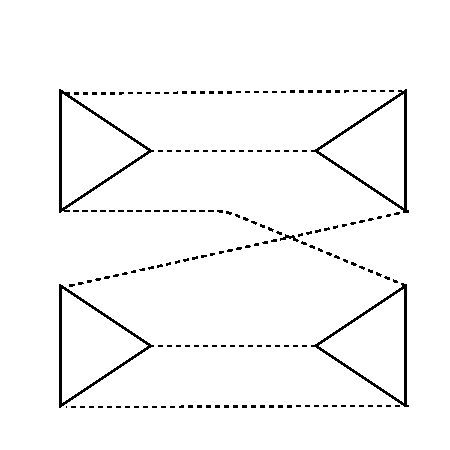
\includegraphics[width=2cm]{AabcBabdCdefDcef}}& 8 & 
		$\tens{A}{_a_b_c}\tens{B}{_a_b_d}\tens{C}{_d_e_f}\tens{D}{_c_e_f}$ & 
		\parbox[c]{3cm}{$\tens{A}{_a_b_c}\tens{B}{_a_b_d} \rightarrow 
			\tens{E}{_c_d}$\\$\tens{E}{_c_d}\tens{C}{_d_e_f}\rightarrow\tens{F}{_c_e_f}$\\
			$\tens{F}{_c_e_f}\tens{D}{_c_e_f}$}  & 
		\SI{0.762(9)}{s}\\
		& 
		& 
		&
		\parbox[c]{3cm}{$\tens{A}{_a_b_c}\tens{B}{_a_b_d} \rightarrow 
			\tens{E}{_c_d}$\\$\tens{C}{_d_e_f}\tens{D}{_c_e_f}\rightarrow\tens{F}{_d_c}$\\
			$\tens{E}{_c_d}\tens{F}{_d_c}$}  & 
		\SI{1.500(4)}{s}\\ \\
		 & 
		 & 
		 &
		\parbox[c]{3cm}{$\tens{A}{_a_b_c}\tens{D}{_c_e_f} \rightarrow 
		\tens{E}{_a_b_e_f}$\\$\tens{B}{_a_b_d}\tens{C}{_d_e_f}\rightarrow\tens{F}{_a_b_e_f}$\\
		$\tens{E}{_a_b_e_f}\tens{F}{_a_b_e_f}$}  & 
		\SI{4.55(4)}{s}\\ \\
		& 
		&
		& 
		\parbox[c]{3cm}{$\tens{A}{_a_b_c}\tens{D}{_c_e_f} \rightarrow 
		\tens{E}{_a_b_e_f}$\\$\tens{E}{_a_b_e_f}\tens{B}{_a_b_d}\rightarrow\tens{F}{_e_f_d}$\\
		$\tens{E}{_e_f_d}\tens{C}{_d_e_f}$}  & 
		\SI{48.4(2)}{s}\\
		\bottomrule
	\end{tabular}
\end{table}





\end{document}